\documentclass[11pt]{article}

\usepackage[margin=1in]{geometry}
\usepackage{amsmath,amssymb,amsthm,mathtools}
\usepackage{booktabs}
\usepackage{graphicx}
\usepackage{microtype}
\usepackage{natbib}
\usepackage{xcolor}
\usepackage{enumitem}
\usepackage{placeins}
\usepackage[hidelinks]{hyperref}
\usepackage[nameinlink,noabbrev]{cleveref}

\definecolor{linkblue}{RGB}{0,80,145}
\hypersetup{colorlinks=true,allcolors=linkblue}
\setlist{nosep,leftmargin=*}
\setlength{\parskip}{0.35em}
\setlength{\parindent}{1.2em}

\newtheorem{theorem}{Theorem}
\newtheorem{proposition}[theorem]{Proposition}
\newtheorem{lemma}[theorem]{Lemma}
\newtheorem{corollary}[theorem]{Corollary}
\theoremstyle{definition}
\newtheorem{definition}[theorem]{Definition}
\newtheorem{assumption}[theorem]{Assumption}
\theoremstyle{remark}
\newtheorem{remark}[theorem]{Remark}

\newcommand{\E}{\mathbb{E}}
\newcommand{\Pp}{\mathbb{P}}
\newcommand{\Var}{\operatorname{Var}}
\newcommand{\ind}{\mathbf{1}}
\newcommand{\doisig}{a_{\epsilon}}
\newcommand{\R}{\mathbb{R}}
\newcommand{\given}{\,\middle|\,}
\DeclareMathOperator{\Bern}{Bernoulli}

\title{Locally Private Causal Inference with Unknown Within-Block Interference:\\
Design-Based Effects, DoI Models, and Minimax Limits}
\author{Anonymous Authors}
\date{}

\begin{document}
\maketitle

\begin{abstract}
Local differential privacy protects each participant before their outcome reaches an analyst,
whereas interference lets one participant's treatment change another's outcome. Combining the
two is not automatic: with a fixed number of arbitrary interference blocks, direct and
spillover effects cannot be estimated with uniformly shrinking uncertainty. We give a
design-based solution for randomized
experiments with independent interference blocks. Blocks are randomized to low or high
treatment saturation, outcomes may depend arbitrarily on every assignment within a block,
and only outcomes are privatized. A one-bit mechanism and Horvitz--Thompson scores identify
saturation-specific direct effects and policy spillover effects without observing or correctly
specifying the latent Degree of Interference (DoI). Cluster-score intervals account jointly for
assignment dependence and privacy noise. For $C$ blocks of $m$ users, the worst-case mean
squared error is, up to design-overlap constants,
$\Theta\!\left(\min\{1,C^{-1}+(Cm\tanh^2(\epsilon/2))^{-1}\}\right)$.
Thus interference limits independent replication while user-level privacy contributes a
separate information loss; multiplying the two penalties would be incorrect. A second oracle
lower bound shows where a multiplicative cost is real: an exposure cell of probability $\rho$
requires risk $\Omega(\min\{1,(Cm\rho\tanh^2(\epsilon/2))^{-1}\})$. The risk grows
exponentially until constant-risk saturation when a DoI cell specifies many peers'
assignments. We also derive the exact privatized-bit likelihood for latent DoI outcome models.
Simulations are consistent with the predicted scaling, show calibrated intervals in a
fixed-population stress test, compare the one-bit mechanism with Laplace noise, and expose the
bias--variance tradeoff of model-dependent outcome regression.
\end{abstract}

\section{Introduction}

Randomized experiments often collect sensitive outcomes in settings where people interact.
A cash-transfer program may affect siblings, a vaccination may protect contacts, and an online
intervention may propagate through a network. Local differential privacy (LDP) asks each user
to randomize their own record before transmission, so the curator never receives the raw
outcome. Interference breaks the usual assumption that a unit's outcome depends only on that
unit's treatment. Each problem is well studied in isolation; together they create a basic
question: what causal effect is still identified, and what information is lost to privacy versus
interference?

Two recent frameworks make the question precise. \citet{OhnishiAwan2025} derive locally
private inference for randomized experiments under no interference. Separately,
\citet{OhnishiKarmakarSabbaghi2025} introduce the Degree of Interference (DoI), a latent random
function that compresses how other units' assignments affect one unit. Their DoI framework
avoids declaring a possibly wrong exposure mapping, but its flexibility necessarily shifts some
work to a model for outcomes given the latent DoI. A direct combination must therefore resolve
three tensions. First, arbitrary interference can prevent concentration even with a large
network \citep{BasseAiroldi2018}. Second, a latent representation cannot create identification
from one observed assignment. Third, privacy noise and assignment dependence enter the risk
through different channels.

We resolve these tensions by separating design-based claims from model-dependent sensitivity
analysis. Our
primary estimands average over randomized saturation policies. The experiment contains $C$
independent blocks of $m$ units. A block is randomized to a low or high treatment probability,
then units are randomized within that block. Interference may be arbitrary and unknown inside
each block, including nonlinear and higher-order effects. This design identifies two direct
effects, one under each saturation policy, and two policy spillover effects, one for treated and
one for untreated units. These quantities do not condition on a learned DoI value. A latent DoI
model is optional: it can improve precision or describe assignment-conditional effects, but it
is not used to justify the main causal identification claim.

The paper makes three claims.

\begin{enumerate}
  \item \textbf{One private bit is enough for design-based inference.} For outcomes in $[0,1]$,
  a tailored one-bit channel gives an unbiased pseudo-outcome. Plugging it into block-level
  Horvitz--Thompson scores \citep{HorvitzThompson1952} yield exactly unbiased direct and
  policy-spillover estimators under
  arbitrary within-block interference. The sample variance of independent block scores gives
  a simple, privacy-aware standard error.

  \item \textbf{Privacy and block interference create two different bottlenecks.} With
  $N=Cm$ users and privacy signal $\tanh(\epsilon/2)$, the matched minimax risk is
  $C^{-1}+[N\tanh^2(\epsilon/2)]^{-1}$, truncated at a constant. The first term counts
  independent interference blocks; the second counts independent local messages. A separate
  oracle bound for a DoI cell of probability $\rho$ is
  $\min\{1,[N\rho\tanh^2(\epsilon/2)]^{-1}\}$. This identifies the genuine
  privacy--interference interaction: rare, highly specific exposures amplify privacy loss
  until risk reaches a constant.

  \item \textbf{Latent DoI models have an exact LDP observation layer.} If an outcome model has
  conditional mean $\mu(z,g)$, the released bit is Bernoulli with probability
  $b_{\epsilon}+\tanh(\epsilon/2)\mu(z,g)$. This likelihood can wrap a dependent Dirichlet
  process or a finite-feature approximation without decoding negative pseudo-outcomes. We use
  a transparent finite-feature outcome regression to show both its possible point-precision
  gain and its
  misspecification risk. This regression is model-dependent and is not used for interval
  inference.
\end{enumerate}

The scope is deliberately narrower than ``arbitrary interference on one network.'' That goal
cannot yield uniformly precise estimation without growing independent replication or
structural assumptions. We require known interference-block boundaries and rule out cross-block
interference; the interference function
inside a block remains unknown. Treatments, block labels, network summaries, and design
probabilities are public. Only each outcome receives an $\epsilon$-LDP guarantee. These limits
are part of the result, not implementation details.

\section{Related work}

\paragraph{Local privacy.}
Randomized response predates modern differential privacy \citep{Warner1965}. Differential
privacy formalized stability to changing one input \citep{DworkMcSherryNissimSmith2006}, and
the local model was connected to statistical-query learning by
\citet{KasiviswanathanEtAl2011}. LDP minimax theory shows that privacy contracts the
distinguishability of nearby distributions \citep{DuchiJordanWainwright2013,
DuchiJordanWainwright2018}. Sharp mechanisms and contraction results appear in
\citet{KairouzOhViswanath2016,KairouzBonawitzRamage2016,AsoodehZhang2024}; broader
geometric and instance-specific views are developed by
\citet{RohdeSteinberger2020,DuchiRuan2024}. Communication reductions and information
contractions give complementary lower-bound tools
\citep{DuchiRogers2019,AcharyaCanonneTyagi2020,BarnesHanOzgur2020,Raginsky2016}.
Locally private mean intervals are studied by \citet{GaboardiRogersSheffet2019}.
\citet{OhnishiAwan2025} are the closest causal reference; their main setting invokes no
interference, whereas our estimands, variance, and lower bounds operate on dependent blocks.

\paragraph{Interference and randomized designs.}
Potential-outcome definitions of direct and indirect effects date at least to
\citet{HalloranStruchiner1995}. Partial interference and two-stage designs make such effects
identifiable \citep{Sobel2006,HudgensHalloran2008,TchetgenTchetgenVanderWeele2012,
LiuHudgens2014,BasseFeller2018}. Randomized saturation and multilevel designs are studied by
\citet{SinclairMcConnellGreen2012,BairdBohrenMcIntoshOzler2018}. Exposure restrictions give
meaning to responses under interference \citep{Manski2013}, and general exposure-based
design estimators are developed by \citet{AronowSamii2017}. Graph-aware designs aim to
increase useful exposure probabilities
\citep{UganderKarrerBackstromKleinberg2013,EcklesKarrerUgander2017}. Randomization tests can
probe interference without fully estimating an effect surface
\citep{BowersFredricksonPanagopoulos2013,AtheyEcklesImbens2018}.

Unknown or misspecified interference is especially relevant here. Unrestricted interference
can defeat large-sample design-based intuition \citep{BasseAiroldi2018}.
\citet{SavjeAronowHudgens2021} characterize what conventional estimators mean under unknown
interference, and \citet{Savje2024} separates effect definitions from exposure restrictions.
Network asymptotics require explicit decay or graph conditions
\citep{Leung2020,Leung2022,LiWager2022}. Other work studies learned networks, network
uncertainty, observational exposures, causal diagrams, treatment-allocation policies, and
bipartite interference
\citep{BhattacharyaMalinskyShpitser2020,ForastiereAiroldiMealli2021,
OgburnVanderWeele2014,PapadogeorgouMealliZigler2019,ZiglerPapadogeorgou2021,
HarshawEtAl2023}. We instead obtain design-based validity by changing the experimental unit of
replication from the person to the interference block.

\paragraph{Latent and Bayesian interference models.}
The DoI framework uses a dependent Dirichlet process mixture to represent an unknown
interference channel \citep{OhnishiKarmakarSabbaghi2025}. Related Bayesian analyses use
generalized propensity scores or flexible models for two-stage experiments
\citep{ForastiereEtAl2022,OhnishiSabbaghi2024}; blocked stick-breaking computation traces to
\citet{IshwaranJames2001}. Our contribution is the LDP observation layer and a clear boundary
between model-based assignment-conditional inference and design-based policy effects.

\section{Setup: latent interference and policy effects}
\label{sec:setup}

\subsection{Randomized saturation design}

There are $C$ interference blocks, indexed by $c$, each containing $m\ge2$ units indexed by $i$;
$N=Cm$. Block $c$ receives a public saturation arm $S_c\in\{0,1\}$ with
\[
  S_c\sim\Bern(r), \qquad r\in(0,1).
\]
Conditional on $S_c=s$, treatments are assigned independently within the block,
\[
  Z_{ci}\mid S_c=s\sim\Bern(p_s), \qquad 0<p_0<p_1<1.
\]
The two values $p_0$ and $p_1$ are the low and high saturation policies. Write
$q_{s1}=p_s$, $q_{s0}=1-p_s$, $r_1=r$, and $r_0=1-r$.

For an assignment vector $\mathbf z_c\in\{0,1\}^m$, unit $(c,i)$ has potential outcome
$Y_{ci}(\mathbf z_c)\in[0,1]$. We make no restriction on how another assignment in the same
block changes this outcome.

\begin{assumption}[Independent blocks and randomized assignment]
\label{ass:block}
Potential-outcome schedules and pretreatment characteristics are independent and identically
distributed across blocks. There is no cross-block interference. The saturation and unit-level
assignments are generated as above and are independent of all potential outcomes.
\end{assumption}

The identical-distribution condition is needed for the superpopulation central limit theorem
and minimax statement. Exact unbiasedness conditional on a fixed collection of $C$ schedules
needs only independent randomization and no cross-block interference.

\subsection{The Degree of Interference is latent}

Let $T_{ci}$ collect public pretreatment information, possibly including a network row. In the
DoI framework, a random function $G_{ci}(T_{ci},\mathbf z_{c,-i})$ compresses other units'
assignments. We use the operational form
\begin{equation}
  Y_{ci}(z,\mathbf z_{-i})
  = \int \widetilde Y_{ci}(z,g)\,
      dF_{ci}(g\mid T_{ci},\mathbf z_{-i}),
  \label{eq:doi}
\end{equation}
where $F_{ci}$ is the latent DoI distribution
\citep{OhnishiKarmakarSabbaghi2025}. Equation~\eqref{eq:doi} includes a deterministic exposure
mapping as a point mass, but does not require one. Our design-based analysis allows
$F_{ci}$ and $\widetilde Y_{ci}$ to be arbitrary inside a block. The DoI is therefore a nuisance
representation for the primary results, not an observed exposure.

\subsection{Direct and policy-spillover estimands}

For $s,z\in\{0,1\}$, define the assignment-marginal cell mean
\begin{equation}
  \mu_{sz}
  = \E\!\left[
      \frac{1}{m}\sum_{i=1}^m
      \E_{\mathbf Z_{c,-i}\sim\Bern(p_s)^{m-1}}
      \{Y_{ci}(z,\mathbf Z_{c,-i})\}
    \right].
  \label{eq:cellmean}
\end{equation}
The outer expectation averages blocks in the target population. The direct effect under
saturation $s$ and the spillover effect of moving from low to high saturation while holding
own treatment at $z$ are
\begin{equation}
  \tau^{\mathrm{dir}}_s=\mu_{s1}-\mu_{s0},
  \qquad
  \tau^{\mathrm{sp}}_z=\mu_{1z}-\mu_{0z}.
  \label{eq:effects}
\end{equation}
These are policy effects: ``spillover'' means changing the distribution of peers' treatments,
not conditioning on a particular latent DoI value. This distinction avoids exponentially rare
exposure cells and gives the estimands meaning even if the latent interference model is wrong.

\begin{proposition}[Why growing block replication is necessary]
\label{prop:replication}
For each contrast in \eqref{eq:effects} under a fixed full-support design with $p_0<p_1$, the
class of bounded arbitrary within-block schedules contains a submodel whose minimax mean
squared error is at least $c/C$, even when raw outcomes are observed. Hence keeping $C$ fixed
precludes uniformly consistent estimation with shrinking uncertainty.
\end{proposition}

The block-shock submodel used in the proof of \cref{thm:minimax} establishes the claim. This is
a precision statement, not nonidentification: the Horvitz--Thompson estimator remains
design-unbiased even at $C=1$, but its worst-case risk cannot vanish. Independent randomized
blocks provide the replication needed for concentration. Other routes are possible, including
structural network decay, but must be stated explicitly
\citep{BasseAiroldi2018,Leung2022}.

\section{Outcome-only local privacy}
\label{sec:privacy}

\begin{definition}[Outcome-only local differential privacy]
A channel $Q$ is $\epsilon$-locally differentially private for the outcome if, for every
$y,y'\in[0,1]$, public design record $d=(S,Z,T)$, and measurable output set $A$,
\[
  Q(A\mid y,d)\le e^{\epsilon}Q(A\mid y',d).
\]
The released messages are conditionally independent across users given the raw experiment.
\end{definition}

This guarantee does not protect $S$, $Z$, $T$, the network, or block membership. It limits
leakage from a participant's own message; correlated neighbors' messages can still reveal
information about that participant, so this is not network or group privacy. Protecting those
variables or inferential channels requires a different mechanism and generally a larger error.

\begin{table}[htbp]
\centering
\caption{\textbf{Scope of the design-based claims.} Here public means available to the analyst
without a privacy guarantee.}
\label{tab:scope}
\small
\begin{tabular}{p{0.23\textwidth}p{0.20\textwidth}p{0.48\textwidth}}
\toprule
Component & Status & Consequence \\
\midrule
Outcome $Y\in[0,1]$ & Private & One noninteractive $\epsilon$-LDP bit per participant \\
Assignment and design & Public & $S,Z,r,p_0,p_1$ enter known inverse-probability weights \\
Blocks and covariates & Public & Block boundaries, $T$, and any network summaries are not protected \\
Interference & Restricted only across blocks & Arbitrary unknown response to every assignment
inside a block; no cross-block effects \\
Primary estimands & Design-marginal & Direct and spillover contrasts average over the two
randomized saturation policies \\
Latent DoI model & Optional & Model-dependent; not required for identification, unbiasedness,
or the cluster-score intervals \\
\bottomrule
\end{tabular}
\end{table}

Define
\[
  \doisig=\tanh(\epsilon/2),
  \qquad b_{\epsilon}=\frac{1}{1+e^{\epsilon}}.
\]
Each user with outcome $Y\in[0,1]$ releases one bit
\begin{equation}
  R\mid Y=y\sim\Bern\!\left(b_{\epsilon}+\doisig y\right).
  \label{eq:mechanism}
\end{equation}
The analyst decodes the bit as
\begin{equation}
  U=\frac{R-b_{\epsilon}}{\doisig}.
  \label{eq:decode}
\end{equation}

\begin{lemma}[Privacy and unbiased decoding]
\label{lem:mechanism}
The channel in \eqref{eq:mechanism} is $\epsilon$-LDP, $\E(U\mid Y)=Y$, and
$\Var(U\mid Y)\le (4\doisig^2)^{-1}$.
\end{lemma}

At $y=0$ and $y=1$, the likelihood ratio for either bit equals $e^{\epsilon}$ in one
direction; every intermediate input is a convex combination. The decoder can be negative or
larger than one, which is harmless: it is only a post-processed estimating variable. As
$\epsilon\downarrow0$, $\doisig\sim\epsilon/2$, recovering the usual $\epsilon^{-2}$ private
mean-estimation cost. As $\epsilon\to\infty$, $\doisig\to1$.

\section{Design-based estimators and inference}
\label{sec:estimation}

For cell $(s,z)$, define
\begin{equation}
  \widehat\mu_{sz}
  =\frac{1}{Cm}\sum_{c=1}^C\sum_{i=1}^m
    \frac{\ind\{S_c=s,Z_{ci}=z\}}
         {r_s q_{sz}}U_{ci}.
  \label{eq:ht}
\end{equation}
The four effect estimators replace each $\mu$ in \eqref{eq:effects} by
$\widehat\mu$. The weights use only known randomization probabilities.

\begin{theorem}[Exact unbiasedness under unknown interference]
\label{thm:unbiased}
Under \cref{ass:block} and \eqref{eq:mechanism}, $\E(\widehat\mu_{sz})=\mu_{sz}$.
Consequently, every direct and spillover estimator is unbiased for its target in
\eqref{eq:effects}. No DoI value, exposure mapping, outcome model, or network is required.
\end{theorem}

For a target contrast $\tau=\sum_{s,z}\ell_{sz}\mu_{sz}$, let the block score be
\begin{equation}
  H_c=\frac{1}{m}\sum_{i=1}^m\sum_{s,z}
  \ell_{sz}\frac{\ind\{S_c=s,Z_{ci}=z\}}{r_s q_{sz}}U_{ci},
  \qquad \widehat\tau=C^{-1}\sum_c H_c.
  \label{eq:blockscore}
\end{equation}
Use the cluster-score variance estimator
\begin{equation}
  \widehat V(\widehat\tau)
  =\frac{1}{C(C-1)}\sum_{c=1}^C(H_c-\widehat\tau)^2.
  \label{eq:variance}
\end{equation}
It automatically includes both assignment covariance inside a block and independent privacy
noise. It does not transplant an independence variance formula from a no-interference setting.

\begin{theorem}[Block central limit theorem]
\label{thm:clt}
Fix $m$, $\epsilon>0$, and design probabilities in $(0,1)$. If the block scores have
nonzero variance, then as $C\to\infty$,
\[
  \frac{\widehat\tau-\tau}{\sqrt{\widehat V(\widehat\tau)}}
  \overset{d}{\longrightarrow}\mathcal N(0,1).
\]
Thus Wald intervals based on \eqref{eq:variance} are asymptotically valid. In experiments we
use the $t_{C-1}$ rather than normal critical value.
\end{theorem}

The theorem is a superpopulation result for iid blocks. Conditional on one heterogeneous
finite collection of schedules, the score variance can include between-block mean
heterogeneity and is generally conservative rather than equal to the finite-population
randomization variance. Our coverage experiment below is therefore a conditional
fixed-population stress test, not a direct proof of the theorem.

\section{Minimax limits: two bottlenecks and an overlap penalty}
\label{sec:minimax}

Let $\eta,\delta>0$, restrict $r,p_0,p_1\in[\eta,1-\eta]$, and require
$p_1-p_0\ge\delta$. Let
$\mathcal P_{C,m}$ contain all independent-block superpopulation laws satisfying
\cref{ass:block} with outcomes in $[0,1]$. For any one contrast in \eqref{eq:effects}, define
the noninteractive outcome-LDP minimax risk
\[
  \mathcal R^*_{C,m}(\epsilon)
  =\inf_{Q\in\mathcal Q_{\epsilon}}\inf_{\widehat\tau}
    \sup_{P\in\mathcal P_{C,m}}
    \E_{P,Q}(\widehat\tau-\tau(P))^2.
\]

\begin{theorem}[Matched privacy--block-interference rate]
\label{thm:minimax}
For constants $0<c_{\eta,\delta}<C_{\eta}<\infty$ depending only on the displayed
design bounds,
\begin{equation}
  c_{\eta,\delta}\min\!\left\{1,\frac1C+\frac{1}{Cm\doisig^2}\right\}
  \le \mathcal R^*_{C,m}(\epsilon)
  \le C_{\eta}\min\!\left\{1,\frac1C+\frac{1}{Cm\doisig^2}\right\}.
  \label{eq:minimax}
\end{equation}
The unprojected estimator in \eqref{eq:ht} is exactly unbiased. Clipping its final contrast to
$[-1,1]$ destroys exact unbiasedness but cannot increase squared error and attains the capped
upper bound.
\end{theorem}

The rate has a useful interpretation. The $C^{-1}$ term is an interference term: an
adversarial schedule can make all $m$ outcomes in a block share one latent shock, so even raw
outcomes provide only $C$ independent draws. The $(Cm\doisig^2)^{-1}$ term is a privacy term:
conditional on the raw outcomes, $Cm$ users still contribute independent privacy coins. These
terms are additive, or equivalently their maximum up to a factor of two. A product
$m/(N\epsilon^2)$ would describe one private message per block, not the user-level privacy
model studied here.

The DoI creates a different penalty when the target conditions on a specific latent exposure.
For fixed $0<\rho\le1$, let $\mathcal E_{N,\rho}$ be the class of iid pairs $(E_i,Y_i)$ with
public exposure labels,
$\Pp(E_i=e)=\rho$, outcomes $Y_i\in[0,1]$, and otherwise unrestricted conditional outcome
laws. The local channel may depend on public $E_i$ but protects $Y_i$. Let
$\mu_e=\E(Y_i\mid E_i=e)$.

\begin{theorem}[Privacy--exposure overlap lower bound]
\label{thm:overlap}
For the oracle-observed exposure problem just defined, the outcome-LDP minimax risk satisfies
\begin{equation}
  \inf_{Q\in\mathcal Q_{\epsilon}}\inf_{\widehat\mu_e}
  \sup_{P\in\mathcal E_{N,\rho}}\E_{P,Q}(\widehat\mu_e-\mu_e(P))^2
  \ge c\min\!\left\{1,\frac{1}{N\rho\doisig^2}\right\}.
  \label{eq:overlap}
\end{equation}
The Horvitz--Thompson one-bit estimator has the matching rate. Since the bound grants the
analyst the true exposure label, it also lower-bounds any procedure that must infer a latent
DoI cell.
\end{theorem}

If $e$ specifies one exact pattern among $d$ independently randomized peers, then
$\rho=p^k(1-p)^{d-k}$. At $p=1/2$, $\rho=2^{-d}$ and the lower bound grows as
$\min\{1,2^d/(N\doisig^2)\}$. The exponential growth before constant-risk saturation is the
genuine multiplicative privacy--interference cost. Policy
means in \eqref{eq:cellmean} integrate over these assignments and avoid conditioning on an
exponentially rare cell. The choice is scientific: exact-exposure effects may be required, but
their information cost should be reported.

\section{An exact LDP likelihood for latent DoI models}
\label{sec:doi}

The design-based estimator answers policy questions without estimating $G$. A scientist may
also want assignment-conditional surfaces or improved point precision. Let a latent DoI model
specify
\[
  G_{ci}\mid T_{ci},\mathbf Z_{c,-i}\sim F_{\phi},
  \qquad
  \E(Y_{ci}\mid Z_{ci}=z,G_{ci}=g,T_{ci})=m_{\theta}(z,g,T_{ci})\in[0,1].
\]
Under the one-bit mechanism, augmentation by $G_{ci}$ gives the exact observation model
\begin{equation}
  R_{ci}\mid z,g,T_{ci},\theta
  \sim\Bern\!\left(b_{\epsilon}+\doisig m_{\theta}(z,g,T_{ci})\right).
  \label{eq:private_likelihood}
\end{equation}
Marginalizing $g$ replaces $m_{\theta}$ by its expectation under $F_{\phi}$. This layer can be
inserted into the dependent Dirichlet process mixture of
\citet{OhnishiKarmakarSabbaghi2025}. It uses the released bit directly, avoids treating the
unbounded decoder $U$ as a Gaussian response, and costs no additional privacy because all
fitting and posterior prediction are post-processing. Equation~\eqref{eq:private_likelihood}
is a unit-level conditional observation layer, not a claim that privatized outcomes are
marginally independent. A full latent model with shared block shocks needs a joint block
likelihood; a product of unit contributions is otherwise a composite likelihood and requires a
block sandwich for uncertainty.

For a transparent empirical sensitivity analysis, we fit a finite-feature outcome regression
rather than the full latent DoI process. Its public dictionary
$\varphi(T,\mathbf Z_{-i})$ contains one-hop and strict two-hop treated fractions, generic
quadratic and cubic terms, a public pretreatment covariate, and own-treatment interactions.
It deliberately excludes the true generating threshold and sinusoidal terms. The conditional
mean is
\[
  m_{\theta}=\operatorname{logit}^{-1}\{\theta^\top\varphi(T,\mathbf Z)\}.
\]
Penalized maximum likelihood under \eqref{eq:private_likelihood} is followed by
g-computation over the two saturation policies. We compare the private fit with the same
generic regression on raw outcomes to isolate privacy loss, and with a no-interference private
regression containing only the public covariate and own treatment. This is a DoI-motivated
observed-feature approximation, not a fit of the latent Dirichlet-process model. None of these
plug-in estimates is design-unbiased, and we do not attach causal confidence intervals to
them; the comparison is a point-risk sensitivity analysis.

\section{Experiments}
\label{sec:experiments}

The experiments ask four questions: (i) Does the one-bit estimator have negligible Monte Carlo
bias and near-nominal coverage under nonlinear unknown interference? (ii) How much does
it improve on outcome-level Laplace noise? (iii) Do sample size, block size, privacy, and exact
exposure probability behave consistently with the predicted rates? (iv) When does
DoI-motivated outcome regression help or hurt point estimation?
All reported points aggregate independent Monte Carlo replications; error bars on RMSE and MSE
are 95\% Monte Carlo intervals, and coverage bars are 95\% Wilson intervals across
replications. The code uses fixed versioned seeds and writes checksums for every result file.

\subsection{Data-generating processes and baselines}

The main nonlinear population has $C=200$ blocks of $m=8$ units. Each block is a ring with
local edges and random chords. Let $e_{1,ci}$ and $e_{2,ci}$ be one-hop and strict two-hop
treated fractions. The latent DoI and bounded potential outcome are
\begin{align*}
  G_{ci}&=0.55e_{1,ci}+0.25e_{2,ci}+0.20\ind\{e_{1,ci}>0.45\},\\
  Y_{ci}(\mathbf z_c)&=\operatorname{logit}^{-1}\bigl[
  -1.15+X_{ci}+0.55z_{ci}+1.10G_{ci}
  +0.35z_{ci}(G_{ci}-0.5)+0.25\sin(2\pi e_{1,ci})\bigr],
\end{align*}
where the fixed public covariate $X_{ci}$ was drawn once from $\mathcal N(0,0.2^2)$. Exact
enumeration of all within-block peer assignments gives the finite-population truth. The design
uses $p_0=0.2$, $p_1=0.8$, and $r=0.5$. We use 800 replications at
$\epsilon\in\{0.25,0.5,1,2,4\}$.

The scaling population uses complete within-block interference and
\[
  Y_{ci}(\mathbf z_c)=0.28+X_{ci}+0.12z_{ci}+0.22\bar z_{c,-i}
  +0.06z_{ci}\bar z_{c,-i}, \qquad X_{ci}\sim\operatorname{Unif}(-0.04,0.04),
\]
so the policy effects are analytic. We vary $C$ at fixed $m=8$, then vary $m$ at fixed
$N=1600$, with 400 replications per condition. The exposure-overlap experiment observes an
exact all-treated peer cell with probability $2^{-d}$, uses $N=100{,}000$ Bernoulli outcomes
of mean $0.6$, and has 2,000 replications. It is an oracle missing-cell subproblem, not a
network simulation: the exposure label is public and own treatment is fixed. The
DoI-feature study uses 150 replications.

Baselines are deliberately matched to the privacy scope: (a) the same design estimator with
raw outcomes; (b) sensitivity-one Laplace noise with the same outcome-only $\epsilon$; and
(c) the released bit without the required debiasing. For the model-based sensitivity study we
compare the design estimator, the generic private-likelihood regression, the same generic
regression on raw outcomes, and a private no-interference regression.

\subsection{Results}

\begin{figure}[htbp]
  \centering
  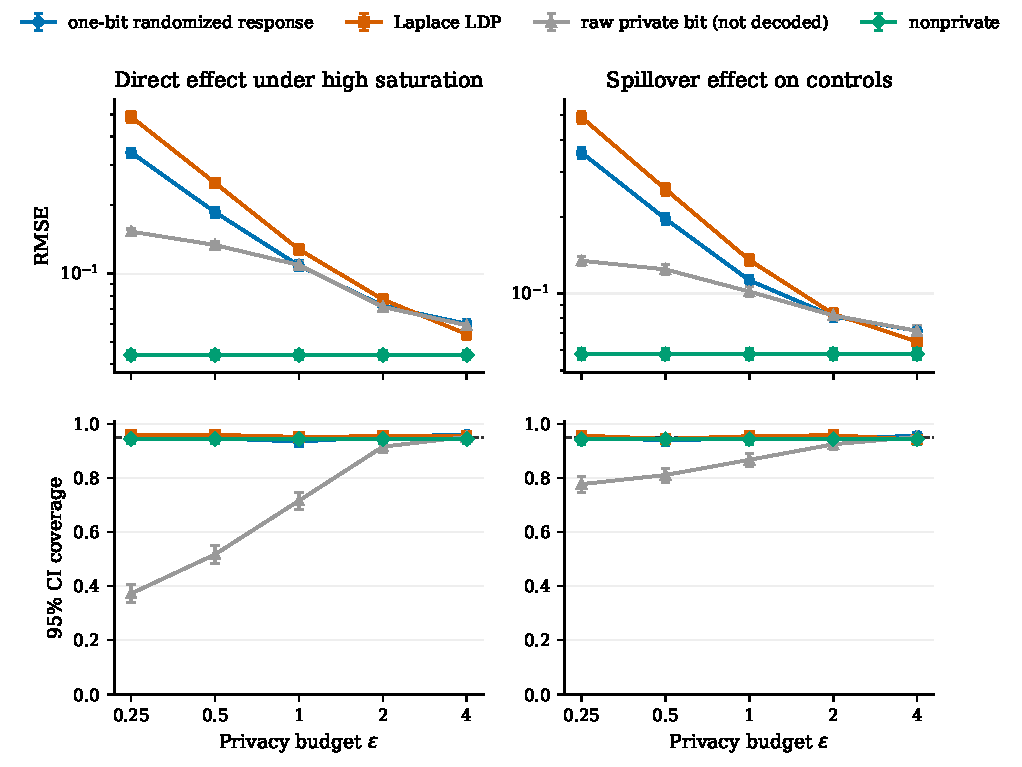
\includegraphics[width=\textwidth]{../figures/privacy_tradeoff.pdf}
  \caption{\textbf{Privacy--accuracy and coverage under nonlinear latent interference.}
  Points show unprojected Monte Carlo RMSE (top) and cluster-score interval coverage (bottom);
  bars are 95\% Monte Carlo or Wilson intervals. The one-bit estimator is unbiased after
  decoding and is most advantageous over Laplace noise at tight privacy. The raw private bit,
  shown only as a negative control, is attenuated toward zero. The dashed line marks 95\%
  coverage.}
  \label{fig:privacy}
\end{figure}

% Generated by scripts/make_tables.py; do not edit by hand.
\begin{table}[htbp]
\centering
\caption{Nonlinear benchmark diagnostics from 800 Monte Carlo replications. Projected RMSE clips only the point estimate to $[-1,1]$; design-based intervals use unprojected cluster scores. SE/SD is the average estimated standard error divided by the empirical standard deviation.}
\label{tab:main}
\scriptsize
\resizebox{\textwidth}{!}{%
\begin{tabular}{lllrrrrrr}
\toprule
Effect & $\epsilon$ & Method & Bias & RMSE & Projected RMSE & SE/SD & Coverage & Mean length \\
\midrule
Direct, high saturation & -- & Nonprivate & -0.000 & 0.044 & 0.044 & 0.97 & 0.945 & 0.169 \\
 & 0.25 & One-bit LDP & +0.007 & 0.341 & 0.341 & 1.04 & 0.955 & 1.405 \\
 & 0.25 & Laplace LDP & +0.016 & 0.489 & 0.466 & 1.02 & 0.960 & 1.975 \\
 & 0.5 & One-bit LDP & +0.014 & 0.186 & 0.186 & 0.99 & 0.948 & 0.729 \\
 & 0.5 & Laplace LDP & +0.003 & 0.250 & 0.250 & 1.01 & 0.960 & 0.995 \\
 & 1 & One-bit LDP & -0.004 & 0.109 & 0.109 & 0.96 & 0.935 & 0.411 \\
 & 1 & Laplace LDP & -0.001 & 0.128 & 0.128 & 1.03 & 0.953 & 0.520 \\
\addlinespace
Spillover on controls & -- & Nonprivate & -0.002 & 0.058 & 0.058 & 0.99 & 0.944 & 0.227 \\
 & 0.25 & One-bit LDP & -0.019 & 0.356 & 0.355 & 1.01 & 0.950 & 1.415 \\
 & 0.25 & Laplace LDP & -0.026 & 0.490 & 0.469 & 1.03 & 0.958 & 1.980 \\
 & 0.5 & One-bit LDP & -0.010 & 0.196 & 0.196 & 0.96 & 0.940 & 0.744 \\
 & 0.5 & Laplace LDP & -0.010 & 0.256 & 0.256 & 0.99 & 0.945 & 1.006 \\
 & 1 & One-bit LDP & +0.001 & 0.113 & 0.113 & 0.98 & 0.946 & 0.438 \\
 & 1 & Laplace LDP & -0.002 & 0.135 & 0.135 & 1.02 & 0.955 & 0.543 \\
\bottomrule
\end{tabular}%
}
\end{table}


Figure~\ref{fig:privacy} supports the first two empirical claims. Across both a direct and a
spillover target, one-bit RMSE falls toward the nonprivate floor as $\epsilon$ grows. At tight
privacy it is substantially smaller than Laplace RMSE, while the raw private bit can look
low-variance only because it is biased toward zero. Cluster-score intervals maintain coverage
near the nominal level in this fixed-population stress test; treating users as independent
would ignore assignment covariance inside blocks.

\FloatBarrier

\begin{figure}[htbp]
  \centering
  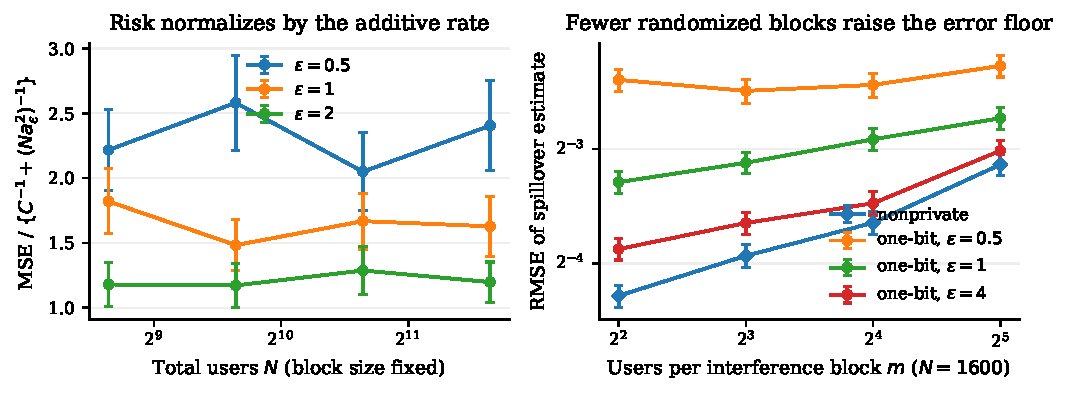
\includegraphics[width=\textwidth]{../figures/rate_scaling.pdf}
  \caption{\textbf{Diagnostics for the two risk components.} Left: observed one-bit MSE divided
  by $C^{-1}+(N\doisig^2)^{-1}$ stays within a budget-specific constant as $N$ and $C$ grow
  with $m=8$. Right: at fixed $N$, increasing $m$ reduces the number of first-stage randomized
  blocks and raises the nonprivate floor, while tight-privacy error is comparatively flat.}
  \label{fig:scaling}
\end{figure}

The normalized risk in the left panel of \cref{fig:scaling} is stable across a fourfold range
of $N$, with no curve fitted to the simulated values. The right panel separates the two
resources hidden by a conventional sample-size label: at fixed $N$, larger blocks mean fewer
first-stage assignments and a larger error floor. This behavior is consistent with the
upper-rate prediction; simulation does not prove the minimax lower bound.

\FloatBarrier

\begin{figure}[htbp]
  \centering
  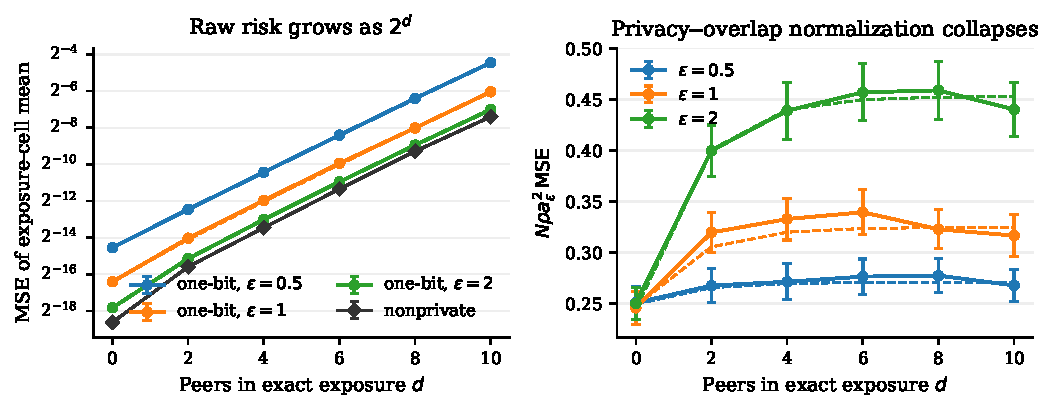
\includegraphics[width=\textwidth]{../figures/exposure_overlap.pdf}
  \caption{\textbf{Privacy multiplies exact-exposure rarity.} An exact assignment pattern among
  $d$ peers has probability $\rho=2^{-d}$. Left: HT mean squared error grows geometrically;
  dashed curves are exact finite-$N$ moment calculations, not fits. Right: the normalized
  quantity $N\rho\doisig^2\mathrm{MSE}$ follows those calculations and is nearly constant in
  $d$ after the dense-cell edge case. Policy-marginal effects avoid selecting this rare cell.}
  \label{fig:overlap}
\end{figure}

\Cref{fig:overlap} illustrates the second lower-bound phenomenon. Every two additional peers
quarter the expected cell count and approximately quadruple MSE. Local privacy shifts each
curve upward by the expected $\doisig^{-2}$ factor; it does not change the geometric dependence
on exposure rarity before constant-risk saturation.

\FloatBarrier

\begin{figure}[htbp]
  \centering
  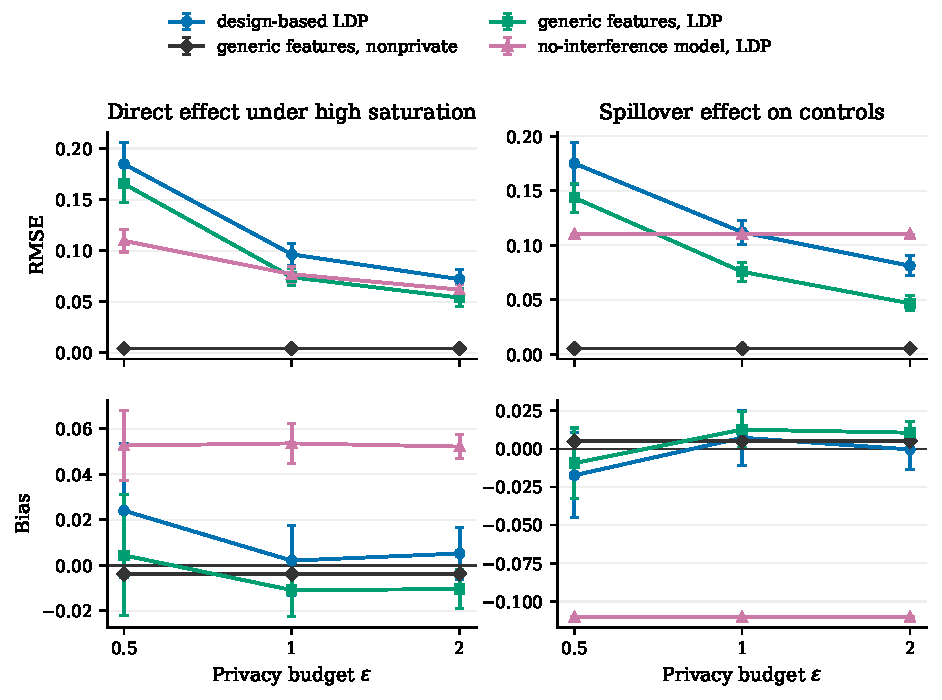
\includegraphics[width=\textwidth]{../figures/doi_sieve.pdf}
  \caption{\textbf{Model-dependent point estimation is a bias--variance choice.} Top: RMSE;
  bottom: signed bias, with 95\% Monte Carlo intervals. Generic polynomial network features use
  the exact privatized-bit likelihood and reduce RMSE here; the same nonprivate fit isolates
  privacy loss. Omitting interference forces the spillover estimate to zero and produces
  persistent bias. Only the design estimator retains a causal guarantee under either model.}
  \label{fig:doi}
\end{figure}

The generic model in \cref{fig:doi} approximates, but does not span, the generating threshold
and sinusoid. It improves point RMSE in this population. The no-interference regression has
smaller direct-effect variance at tight privacy only by accepting bias and estimates the
spillover as zero, $0.110$ below its truth. This is why plug-in fit is not our identification or
interval argument. DoI-motivated models have a complementary role: describe and stabilize a
design-identified policy effect, with feature sensitivity reported.

\FloatBarrier

\section{Limitations and practical guidance}
\label{sec:limitations}

\paragraph{Block boundaries are an assumption.}
The method allows arbitrary interference only \emph{within} known blocks. Cross-block effects
invalidate the independent-block variance and can destroy the growing-replication guarantee.
When approximate interference decay is plausible, network HAC or graph asymptotics may be more
appropriate \citep{Leung2020,Leung2022}.

\paragraph{The privacy scope is outcome only.}
Assignments, block labels, covariates, and any network summaries are public. Jointly protecting
them requires composition or a custom multivariate channel and changes the rate constants.
The one-bit mechanism also assumes a declared outcome range. Clipping an unbounded outcome
changes the estimand unless tail assumptions justify it.

\paragraph{Policy effects are not exact-exposure effects.}
Our spillover effect answers what happens when a block moves from $p_0$ to $p_1$. It does not
answer what happens under one exact peer configuration. \Cref{thm:overlap} quantifies why the
latter may be far harder. Researchers should choose the effect before selecting an estimator.

\paragraph{Latent DoI inference remains model dependent.}
The private likelihood is exact, but a fitted DoI distribution is only as credible as its
outcome model and public interference summaries. We report a misspecification ablation and keep
the design estimator as the primary analysis. Formal Bayesian calibration for a full dependent
Dirichlet process under shrinking privacy is left open.

\paragraph{Large numbers of blocks matter.}
The $t$ interval is asymptotic in $C$, not in the raw user count. A trial with thousands of
users in a handful of interacting villages still has weak design-based replication. Power
calculations should therefore vary both $C$ and $m$, using
$C^{-1}+(Cm\doisig^2)^{-1}$ rather than $N^{-1}$ alone.

\section{Conclusion}

Local privacy does not make unknown interference disappear, and a flexible latent model does
not by itself identify a causal effect. A randomized saturation design changes the situation:
it defines direct and spillover policy effects that average over the unknown DoI, while one
private bit per outcome supports unbiased estimation and cluster-level inference. The minimax
analysis separates two resources---independent blocks and independent local messages---and
shows when they combine additively. Conditioning on a rare DoI cell produces a different,
multiplicative privacy--overlap cost. This distinction is the practical takeaway: design for
policy-relevant marginal effects when possible, report exposure probabilities when not, and use
latent DoI models as transparent sensitivity analyses rather than hidden identification
assumptions.

\appendix

\section{Proofs}
\label{app:proofs}

\subsection{Proof of the privacy lemma}

Let $q(y)=b_{\epsilon}+\doisig y$. Since
$q(0)=1/(1+e^{\epsilon})$ and $q(1)=e^{\epsilon}/(1+e^{\epsilon})$,
$q(1)/q(0)=e^{\epsilon}$. Also
$(1-q(0))/(1-q(1))=e^{\epsilon}$. Both $q(y)$ and $1-q(y)$ are affine, so the largest ratio
over $y,y'\in[0,1]$ occurs at the endpoints. This proves $\epsilon$-LDP. Moreover,
\[
  \E(U\mid Y=y)=\frac{q(y)-b_{\epsilon}}{\doisig}=y,
\]
and
\[
  \Var(U\mid Y=y)=\frac{q(y)\{1-q(y)\}}{\doisig^2}
  \le \frac{1}{4\doisig^2}.
\]

\subsection{Proof of exact unbiasedness}

Condition first on the realized raw outcome. By \cref{lem:mechanism}, replacing $U_{ci}$ by
$Y_{ci}(\mathbf Z_c)$ does not change the expectation. For a fixed unit,
\begin{align*}
&\E\left[
  \frac{\ind\{S_c=s,Z_{ci}=z\}}{r_sq_{sz}}
  Y_{ci}(\mathbf Z_c)
  \right]\\
&\quad=\E_{\mathbf Z_{c,-i}\sim\Bern(p_s)^{m-1}}
  \{Y_{ci}(z,\mathbf Z_{c,-i})\},
\end{align*}
because the inverse probabilities cancel the probabilities of $S_c=s$ and $Z_{ci}=z$.
Averaging units and blocks gives \eqref{eq:cellmean}. Linearity gives the four contrasts.

\subsection{Proof of the block central limit theorem}

Under \cref{ass:block}, the $H_c$ in \eqref{eq:blockscore} are independent and identically
distributed. Fixed positive $\epsilon$ and overlap bound every possible decoded bit and every
weight, so $H_c$ has finite second moment. The iid central limit theorem yields
$\sqrt C(\widehat\tau-\tau)\Rightarrow\mathcal N(0,\Var H_c)$. The sample variance of $H_c$
is consistent for $\Var H_c$, and Slutsky's theorem gives the result. Triangular arrays with
shrinking $\epsilon$ or growing $m$ require a corresponding Lindeberg condition; the fixed
setting stated in the theorem avoids hiding that extra assumption.

\subsection{Proof of the matched minimax theorem}

\paragraph{Upper bound.}
Write $H_c=\E(H_c\mid\mathcal D_c)+\xi_c$, where $\mathcal D_c$ contains the complete raw
block experiment and $\xi_c$ is privacy noise. Bounded raw outcomes and overlap imply
$\Var\{\E(H_c\mid\mathcal D_c)\}\le K_{1,\eta}$. Conditional independence of the local coins,
\cref{lem:mechanism}, and the $m^{-1}$ block average imply
\[
  \E\{\Var(H_c\mid\mathcal D_c)\}
  \le \frac{K_{2,\eta}}{m\doisig^2}.
\]
Independence across blocks then gives
\[
  \E(\widehat\tau-\tau)^2
  \le \frac{K_{1,\eta}}{C}
  +\frac{K_{2,\eta}}{Cm\doisig^2}.
\]
Clipping the estimate to the effect range cannot increase squared error and truncates the bound
at a constant.

\paragraph{Interference lower bound.}
Restrict the parameter class to bounded schedules with
$V_c\stackrel{\mathrm{iid}}{\sim}\Bern(\theta)$ and genuine within-block spillover:
\[
Y_{ci}(\mathbf z_c)
=\frac14+\frac14V_cz_{ci}
+\frac{V_c}{4(m-1)}\sum_{j\ne i}z_{cj}.
\]
The direct contrasts equal $\theta/4$, and the spillover contrasts equal
$(p_1-p_0)\theta/4$. Even an oracle that reveals $V_c$ supplies only $C$ iid Bernoulli draws.
The two-point Le Cam bound therefore gives $c_{\eta,\delta}/C$ risk for every contrast
\citep{Yu1997,Tsybakov2009}. The raw and private experiments are no more informative than this
oracle experiment.

\paragraph{Privacy lower bound.}
Let $W_{ci}\stackrel{\mathrm{iid}}{\sim}\Bern(\theta)$. For a direct contrast, restrict to
$Y_{ci}(\mathbf z_c)=1/4+z_{ci}W_{ci}/4$, whose target is $\theta/4$. For a spillover contrast,
restrict instead to
\[
Y_{ci}(\mathbf z_c)=\frac14+
\frac{W_{ci}}{4(m-1)}\sum_{j\ne i}z_{cj},
\]
whose target is $(p_1-p_0)\theta/4$. Conditional on public assignments, every outcome-LDP
report induces an $\epsilon$-LDP channel of $W_{ci}$ because the outcome is a deterministic
function of $W_{ci}$ and that assignment. Enlarging this induced channel family to all
$\epsilon$-LDP channels of the $N=Cm$ variables $W_{ci}$ can only make estimation easier.
Private Bernoulli mean estimation, with target scaling bounded below by
$\min\{1/4,\delta/4\}$, has risk
$c_{\eta,\delta}\min\{1,(N\min\{\epsilon^2,1\})^{-1}\}$
\citep{DuchiJordanWainwright2018}. Since
$\tanh^2(\epsilon/2)$ and $\min\{\epsilon^2,1\}$ differ only by universal constants, this is
$c'_{\eta,\delta}\min\{1,(N\doisig^2)^{-1}\}$. The maximum of the interference and privacy
lower bounds is at least a constant multiple of their capped sum, completing the proof.

\subsection{Proof of the exposure-overlap theorem}

Condition on the public exposure indicators. Their count $K$ is binomial with mean $N\rho$.
Within the cell, restrict outcomes to Bernoulli distributions whose means differ by a local
two-point perturbation. Conditional on $K$, the LDP contraction bound for Bernoulli mean
estimation gives risk at least $c\min\{1,(K\doisig^2)^{-1}\}$. If $N\rho$ is bounded, the event
$K=0$ has constant probability and the risk is constant. Otherwise, a binomial concentration
event with $K\le2N\rho$ has probability bounded away from zero, giving
$c\min\{1,(N\rho\doisig^2)^{-1}\}$. For the upper bound, use
\[
  \widehat\mu_e=\frac1{N\rho}\sum_{i=1}^N
  \ind\{E_i=e\}U_i.
\]
Its design and privacy variance is $O((N\rho\doisig^2)^{-1})$; clipping to $[0,1]$ gives the
capped rate in the small-cell regime.

\section{Algorithms and reproducibility details}

\paragraph{Primary estimator.}
Each user evaluates \eqref{eq:mechanism} once and sends one bit. The analyst decodes with
\eqref{eq:decode}, computes the four cell scores in \eqref{eq:ht}, forms contrasts, and uses
\eqref{eq:variance}. The unprojected contrast is reported for exact unbiasedness and interval
construction; its clipped version is used for bounded-loss comparisons. No iterative fitting
is involved.

\paragraph{DoI-motivated finite-feature regression.}
We minimize the negative log likelihood from \eqref{eq:private_likelihood} plus an $\ell_2$
penalty of $0.05$ on non-intercept coefficients using L-BFGS. The generic dictionary contains
polynomial rather than true generating bases; the no-interference dictionary omits all peer
summaries. G-computation uses 16 fresh synthetic assignment draws from each target policy.
These draws are post-processing and do not consume privacy budget. These regressions produce
model-dependent point estimates only.

\paragraph{Monte Carlo uncertainty.}
For errors $e_b$ from $B$ replications, RMSE is
$\{B^{-1}\sum_b e_b^2\}^{1/2}$. Its reported Monte Carlo standard error applies the delta
method to the sample variance of $e_b^2$. Coverage bars use Wilson binomial intervals.
All configurations, raw results, summaries, figures, and file checksums are included in the
supplementary repository.

\section{Additional estimand clarifications}

The direct effect $\tau_s^{\mathrm{dir}}$ changes own treatment while averaging peers under the
same policy $p_s$. The policy-spillover effect $\tau_z^{\mathrm{sp}}$ changes peers' assignment
distribution while holding own treatment fixed. Their sum along a path defines a total policy
effect, but we do not report it because the two components are more diagnostic. In general,
$\tau_1^{\mathrm{dir}}\ne\tau_0^{\mathrm{dir}}$ when own treatment interacts with the DoI, and
$\tau_1^{\mathrm{sp}}\ne\tau_0^{\mathrm{sp}}$ for the same reason. The nonlinear simulation was
constructed to include both inequalities.

\bibliographystyle{plainnat}
\bibliography{../references/verified_references}

\end{document}
